\documentclass[twocolumn,showpacs,%
  nofootinbib,aps,superscriptaddress,%
  eqsecnum,prd,notitlepage,showkeys,10pt]{revtex4-1}

% \usepackage[top=1in, bottom=1in, left=1in, right=1in]{geometry}
% \usepackage{times}
% \usepackage{fullpage}
\usepackage{amsmath}
\usepackage{amsthm}

\usepackage{graphicx,wrapfig,lipsum,svg}
%\usepackage{setspace}
%\usepackage{subfig}
\usepackage{hyperref}
\usepackage{xspace}
\usepackage{color}
%\usepackage{flushend}
\usepackage{paralist}
\usepackage[ruled,vlined]{algorithm2e}

\newtheorem{theorem}{Theorem}
\newtheorem{lemma}{Lemma}
% \newtheorem{definition}{Definition}

\usepackage{caption}
\usepackage{tabularx}
\usepackage{enumitem}
\usepackage{thmtools}
\usepackage{thm-restate}

\usepackage{verbatim}

%\usepackage{pstricks}
%\usepackage{pst-node}
%\usepackage{auto-pst-pdf}
%\usepackage{amssymb}
%\usepackage{calc}
%\usepackage{pgffor}
%\usepackage{xparse}
%\usepackage{expl3}
%\usepackage{txfig}

%\begin{figure}
%\begin{pspicture}
%  \drawbox(10.0,-5,0)(n_btc)(tx name)(
%    {$\mathrm{prevTx}_1$,$\mathrm{prevOut}_1$},{$\mathrm{prevTx}_2$,$\mathrm{prevOut}_2$}%
%  )(
%    {lala,lolo},{bli,blo},{adsf,asfd},{$\mathrm{multisig}(2{,}A{,}B)$,$42$~btc}%
%  )
%\end{pspicture}
%\end{figure}

% \setlength{\textfloatsep}{11pt}
% \setlength{\intextsep}{11pt}
% \setlength{\floatsep}{11pt}

% \usepackage{fullpage}

\newenvironment{protocol}[1][tb]
  {\renewcommand{\algorithmcfname}{Protocol}% Update algorithm name
   \begin{algorithm}[#1]%
  }{\end{algorithm}}


\newcommand{\sbline}{\\[\normalbaselineskip]}% small blank line

\newcommand{\authnote}[3]{{ \footnotesize \bf{#1[#2: #3]~}}} % highlighted note
\newcommand{\edit}[1]{\authnote{\color{blue}}{edit}{#1}}

\def\bitcoin{% bitcoin character
  \leavevmode
  \vtop{\offinterlineskip %\bfseries
    \setbox0=\hbox{B}%
    \setbox2=\hbox to\wd0{\hfil\hskip-.03em
    \vrule height .3ex width .15ex\hskip .08em
    \vrule height .3ex width .15ex\hfil}
    \vbox{\copy2\box0}\box2}}

\clubpenalty=10000      % penalty for creating a club line at end of line.
\widowpenalty=10000     % penalty for creating a widow line at top of page.

% Select one or other if want to see comments.
% \com is sometimes displayed during draft.
\long\def\com#1{}
%\long\def\com#1{{\bf \sc comment: }{\small [#1]}{\bf \sc\ endcomment}\newline}

%\long\def\xxx#1{{\bf XXX:} [{\em #1}]}
\long\def\xxx#1{{\color{red} {\bf XXX }{\small [#1]}}}

% Choose abbreviated or long-version alternatives in paper
%\long\def\abbr#1#2{#1}      % abbreviated version
%\long\def\abbr#1#2{#2}     % long version

% Choose abbreviations or long names/titles in bibliography
%\def\bibbrev#1#2{#1}     % short version
\def\bibbrev#1#2{#2}     % long version
%\def\bibbrev#1#2{\abbr{#1}{#2}}   % follow abbr macro

% Abbreviated or full citation lists: \abcite{basic}{others}
%\newcommand{\abcite}[2]{\abbr{\cite{#1}}{\cite{#1,#2}}}

% Conference abbreviations: \bibconf[Nth]{SOSP}{Symposium on ...}
\newcommand{\bibconf}[3][]{#1 \bibbrev{#2}{#3 (#2)}}

% Include page numbers in draft versions only
%\pagenumbering{arabic}

% Workshop/conference version switch
%\long\def\wc#1#2{#1}      % workshop version
%\long\def\wc#1#2{#2}     % conference version

\newcommand{\eg}{{\em e.g.}}
\newcommand{\ie}{{\em i.e.}}

\newcommand{\bmag}{{\bf mag}\xspace}
\newcommand{\sys}{\textsc{Cerberus}\xspace}
\newcommand{\rs}{\textsc{RS}\xspace}

\begin{document}

\title{\sys Channels: \\ Incentivizing Watchtowers for Bitcoin}
% \author{Anonymous
% }
% If the paper title is too long for the running head, you can set
% an abbreviated paper title here
%
\author{Anonymized Submission}
%\author{Zeta Avarikioti\inst{1} \and
%Orfeas Stefanos Thyfronitis Litos\inst{2} \and Roger Wattenhofer\inst{1}}
%
% First names are abbreviated in the running head.
% If there are more than two authors, 'et al.' is used.
%
%\institute{ETH Z{\"u}rich
% \email{\{zetavar,wattenhofer\}@ethz.ch}
%\and
%University of Edinburgh
% \email{o.thyfronitis@ed.ac.uk}
% }
%

%\thispagestyle{empty}

%
%----------ABSTRACT------------
%
\begin{abstract}
Bitcoin and similar blockchain systems have a limited transaction throughput because each transaction must be processed by all parties, on-chain.
Payment channels relieve the blockchain by allowing parties to execute transactions off-chain while maintaining the on-chain security guarantees, \ie, no party can be cheated out of their funds. However, to maintain these guarantees all parties must follow blockchain updates ardently.
To alleviate this issue, a channel party can hire a ``watchtower'' to periodically check the blockchain for fraud on its behalf.

However, watchtowers will only do their job properly if there are financial incentives, fees, and punishments. There are known solutions, but these need complex smart contracts, and as such are not applicable to Bitcoin's simple script language. This raises the natural question of whether incentivized watchtowers are at all possible in a system like Bitcoin.

In this work, we answer this question affirmatively, by introducing \sys channels, an extension of Lightning channels. \sys channels reward watchtowers while remaining secure against bribing and collusion; thus participants can safely go offline for an extended period of time.
We show that \sys channels are correct, and provide a proof-of-concept implementation in the Bitcoin script language.

\keywords{Bitcoin; Security; Payment channels; Payment network; Lightning network; Watchtowers; Collateral; Incentives}
\end{abstract}

\maketitle

%-------------------------------------------------
%---------------INTRODUCTION------------------------
%-------------------------------------------------
\section{Introduction}
\label{sec:intro}

\subsection{Motivation}

Since its inception, Bitcoin~\cite{nakamoto2008bitcoin} is the leading cryptocurrency in terms of market capitalization. Unfortunately, Bitcoin suffers from limited transaction throughput due to its underlying consensus mechanism. Specifically, Bitcoin handles at most 7 transactions/s~\cite{croman2016scaling}, while other payment systems, such as Visa, handle tens of thousands. This is a major obstacle on the wide adoption of Bitcoin.

Payment channels are the foremost solution for scaling decentralized block\-chain systems such as Bitcoin.
They allow transactions between two parties to happen off-chain, while maintaining the security guarantees of the blockchain. Specifically, two parties can open a channel with a single on-chain transaction and then execute multiple transactions privately and off-chain on this channel. The blockchain is only used to close the channel or in case of dispute.

Although payment channels offer a simple and efficient solution to the  limited transaction throughput of blockchain systems, %they also suffer from security issues.
they have a major drawback.
The correct operation of a payment channel depends on all parties of the channel being active and in sync with the blockchain. Otherwise, a party of the channel can close the channel in a wrong state, \ie, a party can publish an outdated version of the channel's funds distribution.
This old state will be considered final,
unless the counterparty disputes it within a specific time period.
% if he counterparty is not active for a long period of time and thus does not dispute the outdated channel state.
This dispute time is chosen when the channel is initiated on-chain; after $t$ blocks, a fraudulent transaction cannot be disputed anymore. Hence, to maintain the security of the payment channel, both parties must be online at least once every $t$ blocks.

A natural solution to relieve the parties from this necessity is outsourcing the dispute process to third-parties, known as watchtowers~\cite{watchtowers,dryja2016monitors}.
Watchtowers on Bitcoin Lightning network~\cite{poon2015lightning} mainly focus on maintaining privacy; however, the current design does not provide incentives for watchtower participation.
In particular, the party that hires the watchtower pays it only if fraud happens. However, the watchtower knows that rational parties never commit fraud, thus there is little incentive to become a watchtower in the first place. Additionally, a rational watchtower can benefit from unintentional broadcasting of revoked updates and thus may lobby for buggy or misleading channel software. A naive alternative would be for the hiring party to pay the watchtower a small fee regularly, \eg, each time a channel transaction is executed. In this case, however, a rational watchtower would avoid the cost of storing the hiring party's data and monitoring the blockchain and would thus fail to act upon fraud.
% In particular, the party that hires a watchtower can either pay the watchtower regularly, \eg, every time a transaction is executed in the channel, or when fraud happens. In the first case, the watchtower can collect the rewards but fail to act upon fraud, so the security of the channel is not guaranteed. In case the watchtower is paid upon fraud only, the watchtower risks to never be paid, and hence has little incentive to be a watchtower in the first place. Additionally, a rational watchtower in the latter case can benefit from unintentional broadcasting of revoked updates and thus may lobby for buggy or misleading channel software.

In this paper, we introduce \sys channels, where watchtowers are (i) incentivized to participate in the system, and (ii) penalized in case they do not act upon fraud.
In particular,
%in \sys channels,
each party has the option to employ a watchtower as a service provider. The watchtower  is paid for every transaction executed on the channel and locks collateral on-chain as guarantee for its honest behavior. In case the watchtower misbehaves and does not dispute an outdated state, the cheated party can claim the watchtower's collateral.
Hence, rational watchtowers are incentivized both to participate and act upon fraud.
In our construction, the parties can go offline for an extended period of time and need only be online to penalize the watchtower.
This way we weaken the availability requirement for the parties of a payment channel.
More importantly, \sys channels build upon and extend Lightning channels and only require timelocks and additional transactions.% and hashlocks.
We also provide a proof-of-concept implementation (\url{https://github.com/fc-submission-132/cerberus-script}).

% Other channel constructions are available that provide incentive-compatible solutions~\cite{avarikioti2019brick,mccorry2018pisa}; none of them however are compatible with script and thus cannot be deployed on Bitcoin.

\subsection{Related Work}
\label{sec:related}
% Payment channels are the most prominent solution to the scalability problem of current blockchain systems.
Payment channels were first introduced by Spilman \cite{spilman2013channels} as unidirectional channels and were later established as bidirectional channels \cite{poon2015lightning,decker15fast}. Currently, there exist a variety of bidirectional payment channels constructions, some applicable only on platforms that allow for arbitrary smart contracts such as Ethereum \cite{dziembowski2017perun,Miller2017sprites,green2017bolt,avarikioti2019brick}, and some applicable also on blockchain systems with limited scripting languages like Bitcoin \cite{poon2015lightning,deckereltoo,decker15fast,avarikioti2018watchtowers}. This work falls in the second category.
% ; \edit{remove "we introduce \sys, a new payment channel construction, and provide a proof-of-concept implementation on Bitcoin."}

The most famous and active payment network is Lightning \cite{poon2015lightning} currently operating more than $35,900$ channels by over $9,900$ nodes with a sum of more than $830\bitcoin$~\cite{lightning-stats}. However, Lighting as well as most of the other payment networks require channel parties that are frequently online, watching the blockchain. To address this issue, Dryja introduced Monitors \cite{dryja2016monitors}, also known as Watchtowers~\cite{watchtowers}, a third-party solution that acts as a proxy for a channel's party effectively allowing the party to go offline for a long period of time while maintaining the security of the channel (the other party cannot cheat). Watchtowers mainly focus on privacy preserving techniques to ensure the hired third-party does not learn any information about the off-chain transactions.
Thereafter, DCWC~\cite{avarikioti2018watchtowers} was proposed, a distributed protocol for watchtower services, in an attempt to involve all full nodes in the system and consequently enhance security.
However, both these works, Watchtowers and DCWC, fail to provide the necessary incentives for participation in the system.
In particular, the watchtowers are paid upon fraud. Thus, since no rational party will commit fraud, watchtowers will never be paid.
% Therefore, there will be no watchtowers.
Therefore, assuming rational participants, the existence of watchtowers is not a Nash equilibrium.
% In particular, if a party hires watchtowers and pays them regularly, the watchtowers have no incentive to do their job (since they are paid regardless). On the other hand, if the watchtowers are paid upon fraud, they will not participate in this system because no rational party will commit fraud hence they will never be paid. Thus, there will be no watchtowers.
On the contrary, \sys channels provide the necessary incentives mechanisms for watchtowers (rewards and punishment).
% , \edit{remove "\ie, penalization of the watchtower's collateral in addition to the occasional rewards"}.

In the same vein, McCorry et al.\ presented Pisa~\cite{mccorry2018pisa}, a protocol that outsources the dispute handling of (state\footnote{State channels generalize payment channels to support smart contracts~\cite{Miller2017sprites}.}) channels to third-parties. However, Pisa has two shortcomings: First, the main protocol implementation is not secure against bribing since the watchtower's collateral is not linked to the party or the channel on-chain, hence the watchtower can double-spend it. Second, Pisa is not compatible with Bitcoin, because it requires a smart contract not expressible in script. On the contrary, \sys channels are applicable to Bitcoin and furthermore they do not suffer from the security problems of Pisa since the watchtower's collateral is linked to the hiring party with an on-chain transaction.
% the watchtower locks the collateral linked to the hiring party on-chain".

More recently, Avarikioti et al.\ introduced Brick~\cite{avarikioti2019brick}, an asynchronous off-chain construction that employs a committee of watchtowers. Although Brick manages to remove the synchrony requirements on the network layer and the perfect blockchain assumption while maintaining the security of channels, it is not compatible with Bitcoin-like platforms, as opposed to \sys channels.
% \edit{remove "In this work we provide a proof-of concept implementation on Bitcoin, which can be found in Appendix~\ref{sec:script}"}.

In a different line of work, Khabbazian  et al.~\cite{khabbazian2019outpost} proposed a lightweight watchtower design in which watchtowers do not need to store the signed justice (revocation) transactions, but instead can extract them  directly from the commitment transactions that appear on the blockchain.
This work is independent and complementary to ours, and can be applied also to \sys channels to improve the storage requirements for the watchtower service.
% This work is independent to ours, since it considers the original watchtower proposal \cite{dryja2016monitors} that due to privacy reasons
% requires large storage and lookup time for the watchtower.
% In contrast, off-chain transactions in \sys are not hidden from then watchtowers.

\subsection{Our contribution} To summarize, the contribution of this paper is the following:
\begin{itemize}

    \item We introduce \sys payment channels that
enable participants on Bitcoin to employ watchtowers and thus go securely offline for an extended period of time.
% allow watchtowers to lock collateral tied to the channel construction, effectively securing the channels when channel parties are offline for an extended period of time.
    \item We define the desired properties for payment channel solutions and prove \sys channels are secure under our security model. Specifically, we show  watchtowers are incentivized to both participate and act upon fraud. Thus, \sys channels are secure against collusion and bribing.
    \item We provide a proof-of-concept implementation of \sys channels on Bitcoin (Appendix \ref{sec:script}).
\end{itemize}

% Omitted proofs and a proof-of-concept implementation of \sys channels on Bitcoin can be found in Appendix \ref{sec:proofs} and \ref{sec:script}\footnote{The implementation can be found at \url{https://github.com/fc-submission-132/cerberus-script}.}, respectively.

%-------------------------------------------------
%---------------BACKGROUND------------------------
%-------------------------------------------------
\section{Background and Notation}
\label{sec:back}
% In this section, we introduce the necessary primitives and notation that our construction builds upon.
\subsection{Payment Channels}
For the rest of the paper, when we refer to payment channels we imply Lightning channels, currently operating on the Bitcoin network.
We now provide a brief overview of Lightning channels, on which \sys channels build upon.

To open a payment channel, the parties publish a funding transaction where they lock their funds into a common account, \ie, both parties must sign to spend the output of the funding transaction. Every time the parties execute a transaction, they update the current state of the channel accordingly, meaning they distribute the funding transaction's output as agreed and sign  the resulting ``commitment'' transaction. In addition, each party reveals to the counterparty a secret that allows the counterparty to  sign a ``revocation'' transaction that spends the previous commitment transaction; the revocation transaction awards  the cheating party's funds to the cheated party, effectively punishing the party that tried to cheat.
The output of the party that published the commitment transaction is locked for a time period, known as the revocation period. The cheated party must publish the revocation transaction during the revocation period, otherwise the  cheating party will be able to spend the balance of the revoked state. Thus the security of the channel construction  crucially depends on all parties of the channel watching the blockchain and being online at least once during the revocation period.

% \edit{remove the whole paragraph?} To address this problem, third parties, known as watchtowers~\cite{watchtowers,dryja2016monitors}, were introduced. A watchtower acts as a proxy for the party that hires him, allowing the party to go offline for a long period of time. In particular, in case the counterparty attempts to close the channel in a previous state, the watchtower acts on behalf of the offline party and publishes the revocation transaction.

% The watchtowers on the Lightning protocol mainly focus on maintaining privacy; however, the current design does not provide incentives for participation for the watchtowers. In particular, the party that hires a watchtower can either pay the watchtower every time a channel update occurs or when fraud happens. In the first case, the watchtower can collect the rewards without acting upon fraud, so the security of the channel is not guaranteed. In case the watchtower is paid upon fraud, the counterparty knowingly-so will not commit fraud,  thus the watchtower will not be paid and hence is not incentivized to participate.

% To address this issue, we introduce \sys channels, where watchtowers are incentivized to participate in the system and are penalized in case they do not act upon fraud. Other channel constructions are available that provide incentive-compatible solutions~\cite{avarikioti2019brick,mccorry2018pisa}; none of them however are compatible with Bitcoin script and thus cannot be deployed on Bitcoin.




%----------------------CONTRACTS--------------------------------------
\subsection{Contracts}
A contract is an agreement that can be enforced on the blockchain.
Enforcing such a contract depends on the operations the programming language allows with respect to transaction outputs.
Most recent cryptocurrencies, such as Ethereum, support a
Turing-complete language and thus can enforce arbitrary rules with a \textit{smart contract}. However, Bitcoin (as well as other cryptocurrencies) has strict limitations on the scripting language and allows only specific operations. As a result Bitcoin's contracts are simpler and with limited functionality.
Next, we discuss the operations allowed in script with respect to transaction outputs, on which \sys channels build upon.

\paragraph{Signatures.} A signature is the most basic form of contract and is essentially a proof of ownership of a transaction output. We denote by $\sigma_A$ the signature that corresponds to the public key $A$. (We omit the signed message, as it always is the transaction which contains the signature, with a placeholder in the location of the signature).
Further, an $m$-of-$n$ \textit{multisignature} is a contract that demands at least $m$ signatures which correspond to  any $m$ of the $n$ predefined public keys.
% For instance, $\sigma_{A,B,C}^2$ denotes a 2-out-of-3 multisig for the public keys $A, B$ and $C$.
If $m$ valid signatures are provided then the output is immediately spendable.
 In this work, we will only use 2-of-2 multisignatures, so we introduce the following notation: $\sigma_{A,B}$ expresses that the output of the transaction can only be spent with both the signatures of $A$ and $B$.

\paragraph{Timelocks.} Timelocks are another type of contract. When a transaction or a transaction output is timelocked it cannot be included in the blockchain until the specified time has elapsed. There are two types of timelocks, \textit{absolute}~\cite{bip65} and \textit{relative}~\cite{bip68}. Transactions or transaction outputs with an absolute timelock become valid when the specified timestamp or block height is reached. On the other hand, a relative timelock allows a transaction output to be locked for a time relative to the block that included that output.
Relative timelocks are used in the Lightning  protocol as well as in our protocols.
% This type of timelock is used in the Lightning network and will also be used in our protocols.
We denote by $\Delta t$ a relative timelock that expires $t$ blocks (confirmations) after the transaction is included in the blockchain. After this time the output of the transaction is spendable.


% \paragraph{Hashlocks.} \edit{remove entire paragraph -- hashlocks not used in \sys}
% % Hashlocks are another type of contract, available also in Bitcoin Script.
% If a transaction output is hashlocked, it requires the pre-image of the specific hash to become valid and thus spendable. For instance, suppose $h(s)$ denotes the hash of a secret $s$. If an output is hashlocked with $h(s)$, it is valid only if the secret $s$ is revealed.

%----------------------UTXO NOTATION--------------------------------------
\subsection{UTXO Notation}
In this section we introduce the necessary notation for our protocol.

We assume the blockchain is UTXO-based (UTXO: Unspent Transaction Output), meaning that transactions consist of inputs and outputs.
A transaction  connects its inputs to UTXOs (removing the latter from the UTXO set) and creates new UTXOs, its outputs.
% A transaction takes UTXOs as inputs, destroys them, and creates new UTXOs, the outputs.
Each UTXO can only be spent as a whole. A UTXO consists of a monetary value and the conditions under which it can be spent, \eg, a signature corresponding to a public key, a timelock etc.

We denote by $o=(x \mid C)$
the UTXO that holds a monetary value of $x$ coins that can be spent when conditions $C$ are met. For example, $o=  (10 \mid \sigma_A)$ means that the signature that matches the public key A can spend the output $o$ which is equivalent to 10 coins.

A transaction in this model is a mapping from a set of UTXOs, called inputs, to a (new) set of UTXOs, called outputs.
We define a transaction as follows:
$$TX_i= [o_j, o_k, \dots] \mapsto [o_i^1, o_i^2, \dots] $$
where $o_j$, $o_k$, etc.\ are the inputs of the transaction and $o_i^1, o_i^2, \dots $ are the first, second, etc.\ outputs, respectively.
% Note that we refer to the $l$th (output) UTXO of a transaction $TX_i$ as $o^l_i$.
If transaction $TX_i$ has a single output we simply write $o_i$.
Moreover, if the specific UTXO that is input to a transaction is irrelevant to the protocol design, we refer to it as ${\#}$. If we demand the input to belong to a specific public key $A$ and hold a specific value of $x$ coins, but which of the UTXOs owned by $A$ is spent by the input is irrelevant to the protocol design, we refer to it as $(x \mid {\#}_{\sigma_A})$.
For instance,
$$TX_{i}= \big[(0.8 \mid {\#}_{\sigma_A}), o_k^2\big] \mapsto \big[(1 \mid h(s)), (0.5 \mid \sigma_B)\big]$$
denotes the transaction $TX_i$ that spends a UTXO from the party $A$ with value $0.8$ coins and the second output of transaction $TX_k$ and creates two new UTXOs. The first output holds the value of $1$ coin and can be spent with the secret $s$, while the second holds $0.5$ coins and can be spent with $B$'s signature.





%-------------------------------------------------
%---------------MODEL------------------------
%-------------------------------------------------
\section{Protocol Overview}
%----------------------MODEL--------------------------------------
\subsection{System Model}\label{subsec:model}

\paragraph{Cryptographic Assumptions.}
We make the typical cryptographic assumptions, \ie, there are secure communication channels between participants, and cryptographically secure hash functions, signatures, and encryption schemes. Additionally, all parties of the protocol (watchtowers, channel parties, external adversaries) are computationally bounded.

\paragraph{Blockchain Assumptions.}
We assume a perfect blockchain, in the sense that both persistence and liveness hold~\cite{garay15bitcoin}. In particular, we assume that if a valid transaction is propagated in the blockchain network it cannot be censored and will be included in the ``permanent'' part of the blockchain immediately\footnote{Note that \sys channels can be made secure for any confirmation time $k$, but we choose $k=1$ to simplify the protocol and security analysis.}.

\paragraph{Network Model.}
We assume that any participant of a channel can go offline (intentionally or due to a Denial-of-Service (DoS) attack) for a (long) period of time up to $T$. Furthermore, we consider watchtowers that are resilient against DoS attacks. We argue this assumption is realistic since watchtowers are also required to lock high collateral to participate in the system and thus operators will invest in anti-DoS protection.

\paragraph{Threat Model.}
We assume that the watchtowers as well as the channel participants are rational players. Thus, they will only deviate from the honest protocol execution if they can gain more profit. Moreover, channel participants can collude with the watchtower(s).



%----------------------OVERVIEW--------------------------------------
\subsection{\sys Overview}
\sys channels aim to alleviate the need for the channel parties to be frequently online watching the blockchain.
% Currently on Bitcoin, parties that operate a Lightning channel must be online during the revocation period $t$ to ensure the security of the channel. The watchtower implementation of Lightning that outsources the dispute resolution to third-parties is not secure since incentives are not aligned.
We propose simple modifications on the Lightning protocol that  allow the  parties to employ watchtowers while incentives for active participation and thus security of the channels are guaranteed.

In particular, in \sys, the watchtower is rewarded for every update on the channel but also locks collateral as guarantee for the case he does not act upon fraud. The party employing the watchtower can claim the collateral within the penalty period, if the latter misbehaves. The penalty period is however much larger than the revocation period, hence the hiring party can go offline for an extended period of time.
On the other hand, on a normal operation of the channel the watchtower can reclaim the collateral when its service is terminated.
The watchtower has the option to terminate its service to the party at any point during the protocol execution subject to the penalty period. In such a case, the party can either update the channel and employ a new watchtower, close the channel, or be online more frequently to avoid fraud.

%During every update the watchtower signs a penalty transaction that is tied to the previous commitment transaction. Furthermore, the revocation transaction is modified to spend both outputs of the funding transaction.
%Thus, if fraud occurs, meaning a previous commitment transaction is published on-chain, and the watchtower does not publish the corresponding revocation transaction, the party employing the watchtower can claim the collateral. Hence, a rational watchtower is incentivized to publish the revocation transaction and thus a rational party will not cheat.

%----------------------GOALS--------------------------------------
\subsection{Payment Channel Properties}\label{subsec:goals}
We define the desired properties of a payment channel construction below, summarizing the work of \cite{mccorry2018pisa,Miller2017sprites,avarikioti2019brick,gudgeon2019sok}.

\begin{enumerate}
    \item \textbf{Security:} Any party of the channel can enforce the last agreed state (balance) on-chain at any time.
    %\item \textbf{Watchtower Security:} An honest watchtower can eventually spend on-chain at least the entire collateral when the channel closes or when it activates \textit{Abort}.
    %\item \textbf{Party Security:} An honest channel party can eventually spend on-chain at least their channel balance as defined by the latest \textit{Update} when the channel closes.
    \item \textbf{Privacy:} No third-party, external to the payment channel, can gain information about the state (distribution of funds) of the channel.
    \item \textbf{Scale-out:} The number of transactions on-chain is constant.
\end{enumerate}

The first two, namely Safety and Privacy, are security properties, while the third is the performance property that is required in a channel to achieve its main purpose -- higher transaction throughput.
%We will later show that \sys achieves all these properties.

We note that these properties are also met by Lightning, but under a different network model. Specifically, Lighting requires participants to be frequently online watching the blockchain to guarantee security. In this work, we aim to alleviate this requirement, thus providing security as specified in Section~\ref{subsec:model}.






%-------------------------------------------------
%---------------SYSTEM------------------------
%-------------------------------------------------
\section{\sys Design}\label{sec:design}

In this section, we describe in detail the architecture of \sys payment channels. We base our design on Lightning channels, and introduce the necessary modifications and extensions to guarantee the desired properties under the predefined model for our design and the applicability to Bitcoin.

First, we divide the channel lifetime in four phases: \textit{Open, Update, Abort} and \textit{Close}. Then, we describe the necessary transactions  and present the protocol design for each phase.
To simplify the description, we assume, wlog, that party $B$ has hired watchtower $W$ and the potentially cheating party is $A$.

We note that \sys can accommodate the usecase where only one party wishes to hire a watchtower, as well as that in which both parties choose to do so. Different watchtowers can be used by the two parties. In the case neither party employs a watchtower, the protocol reverts to Lightning.


\subsection{Phase: Open}\label{subsec:open}
% \edit{remove "The first phase, \textit{Open}, is the setup phase of opening a channel."}
Similarly to the Lightning protocol, phase \textit{Open} includes a funding transaction and a commitment transaction.
The funding transaction creates a common account between the parties and is eventually published on-chain to notarize the committed funds, hence the opening of the channel. The funding transaction of a \sys channel spends the funds of the channel parties and creates a new 2-of-2 multisig output spendable only if the parties collaborate.

The commitment transaction (first of many to follow) distributes the funds between the  parties and is signed and held in private by both parties. The commitment transaction, if published, does not allow the publishing party to spend its funds immediately, to ensure there is enough time for punishment in case of fraud (\ie, the commitment transaction is not the last agreed state by the channel parties). This is known as the revocation period, denoted by $t$. The first commitment transaction should be signed by both parties before signing and publishing the funding transaction to avoid a hostage situation.

Furthermore, we introduce two new transactions in phase \textit{Open}, the \textit{collateral transaction} and \textit{reclaim transaction}, that involve the watchtower service.
The collateral transaction is funded by the watchtower, while its output is a joint account between the watchtower and the hiring party. The value of the collateral is slightly higher than the channel funds.
The reclaim transaction, on the other hand, allows the watchtower to reclaim the collateral, effectively terminating its service.
The output of the reclaim transaction can be spent as follows: either a long ``penalty'' period $T$ has elapsed since the watchtower signed and published on-chain the reclaim transaction, or both the signatures of the watchtower and the party are present.
Intuitively, the penalty period $T$ allows the cheated party to penalize an inactive/malicious watchtower, during phase \textit{Close}. Further, timelock $T$ allows the party employing the watchtower to be notified either in case of fraud or in case the watchtower simply wants to withdraw its service. In the latter case, the party can either be online more frequently (revocation period), close the channel, or collaboratively update the channel to cancel out the previous commitment transactions and employ a new watchtower.
% Intuitively, the penalty period $T$ allows the cheated party to penalize a malicious watchtower that did not act when fraud happened, during phase \textit{Close}. Further, the timelock $T$ allows the party employing the watchtower to be notified either in case of fraud or in case the watchtower simply wants to withdraw its service. In the latter case, the party can either be online more frequently (revocation period), or close the channel, or collaboratively update the channel to cancel out the previous commitment transactions and potentially employ a new watchtower. On the other hand, the collateral cannot be spent by the party since the signature of the watchtower is necessary.
% We will later show that the timelock $t$ ensures that the party employing the watchtower cannot cheat by claiming the  collateral of an active watchtower.
Note that the reclaim transaction is signed by both the watchtower and the hiring party before the collateral transaction is put on-chain to avoid a hostage situation.

Further, $T>>t$, and security holds as long as any participant in a \sys channel employing a watchtower is offline for at most $T$ time.

Next, we present in detail the transactions involved in the first phase, \textit{Open}.%, which is described in Protocol~\ref{prot:open}.
% We assume, without loss of generality, that party $B$ hires watchtower $W$.
\begin{itemize}
    \item \textbf{Funding transaction:} Opens a channel between two parties, $A$ and $B$. The inputs are the parties' funds and the output is a 2-of-2 multisig of $A$ and $B$.

     \item \textbf{Commitment transaction:} Updates the state of the channel, \ie, the distribution of the funds between the parties. The input of the commitment transaction spends the output of the funding transaction. The commitment transaction has two outputs, one for each channel party, and distributes the funds of the channel to the two parties as agreed. Each party has its own version of the commitment transaction, signed by the counterparty. Each version has two outputs, one awarded to the party holding the commitment transaction, wlog party $A$, and one awarded to the counterparty $B$.
     Both outputs are timelocked for the revocation period $t$. Further, each output can be spent before $t$ time elapses in collaboration with the watchtower $W$, \ie, if both the watchtower and the corresponding party sign a transaction.
    %  one output awarded to the party holding the commitment transaction, wlog party $A$, with the following conditions: either the signature of $A$ timelocked (for the so-called revocation period, $t$), or the signature of $A$ and the watchtower $W$. Additionally, the same version of the commitment transaction includes a second output that can be spent by $B$ timelocked by $t$ or by the signature of both $B$ and the watchtower $W$.
    \item \textbf{Collateral transaction:} Commits the watchtower's collateral on-chain. Note that the value of the collateral should be slightly higher than the total funds of the channel. The input of the collateral transaction is funded by the watchtower, while the output is a 2-of-2 multisig of $B$ and $W$.
    \item \textbf{Reclaim transaction:} Allows the watchtower to reclaim the collateral. The input of the reclaim transaction spends the output of the collateral transaction.
    The output, on the other hand, requires the signature of the watchtower relatively timelocked by $T$ or both the signatures of $W$ and $B$.
\end{itemize}


\begin{figure*}[ht!]
	\fbox{
	\begin{minipage}{0.97\textwidth}
	\begin{flushleft}
	\noindent\textbf{Protocol: Open}\\
	\noindent\emph{Preconditions:} $A, B$ and $W $ own on-chain $a, b$ and $c$ coins respectively. It holds that $c>a+b$ and $W$ is employed by $B$.

    \noindent $A$ and $B$ prepare the necessary transactions.
	\begin{enumerate}
        \item $A$ and $B$ create the funding transaction:
        $TX_f= \big[(a \mid {\#}_{\sigma_A}), (b \mid {\#}_{\sigma_B})  \big] \mapsto (a+b \mid \sigma_{A,B}) $
        \item $A$ and $B$ create the first commitment transaction (version held by $A$):\\
        $TX_{C1A}= o_f \mapsto \big[(a \mid ({\sigma_A} \wedge \Delta t) \vee \sigma_{A,W}), (b \mid  ({\sigma_B} \wedge \Delta t) \vee \sigma_{B,W})  \big] $
    \end{enumerate}

    \noindent $A$ and $B$ open the channel.
    \begin{enumerate}[resume]
        \item $B$ sends the signature of $TX_{C1A}$ to $A$.
        Symmetrically, $A$ sends the signature of $TX_{C1A}$ to $B$.
        \item Both $A$ and $B$ sign $TX_f$ and publish it on-chain, as in Lightning.
    \end{enumerate}

    \noindent $W$ locks its collateral for the channel on-chain.
    \begin{enumerate}[resume]
        \item $W$ creates the collateral and reclaim transactions and sends both to $B$:\\
        $TX_{\mathit{Coll}}= (c|{\#}_{\sigma_W}) \mapsto (c \mid \sigma_{W,B})$\\
        $TX_{RC}= o_{\mathit{Coll}} \mapsto (c \mid (\sigma_{W}\wedge \Delta T) \vee (\sigma_{B,W}) ) $

        \item $B$ verifies, signs and sends to $W$ the signature for the input of $TX_{RC}$.
        \item $W$ signs and publishes on-chain the collateral transaction $TX_{Coll}$.
    \end{enumerate}

    \noindent\emph{Postconditions:} Opening of the channel between $A$ and $B$ with total value $a+b$ coins, and employment of $W$ from $B$ with $c$ coins as collateral.
        \end{flushleft}
	\end{minipage}
	}
% \caption*{Opening of a \sys channel}
% \label{prot:open}
\end{figure*}

\subsection{Phase: Update}\label{subsec:update}

The second phase, \textit{Update}, % described in Protocol \ref{prot:update},
materializes the main functionality of a channel. In this phase, the parties update the current state of the channel (distribution of funds) and consequently transactions are executed off-chain. The \textit{Update} phase in the Lightning protocol consists of a (new) commitment transaction and a revocation transaction. The commitment transaction represents the last, agreed by both parties, state of the channel. On the other hand, the revocation transaction allows a party to claim all the funds of the channel in case the other party publishes the previous commitment transaction (attempts to cheat).

The \textit{Update} phase in \sys produces the following transactions: a commitment transaction, a revocation transaction, and two penalty transactions.
% Every time the parties want to update the channel's state by issuing a new commitment transaction, the aforementioned transactions must also be created to ensure the alignment of incentives that guarantee the security of the construction.
The revocation transaction spends both outputs of the previous valid commitment transaction and awards them to the cheated party $B$.
The revocation transaction is signed by the potentially cheating party $A$ and is sent to $B$.
%This transaction is signed  by the potentially cheating party and sent to the counterparty.
Then, both party $B$ and watchtower $W$ sign, exchange and store the revocation transaction.
Note that $B$ will not sign the new commitment transaction unless both $A$ and $W$ sign the revocation transaction.
Further, $A$ acts as in Lightning.

The penalty transactions allow $B$ to penalize watchtower $W$ during the penalty period in case fraud occurred and $W$ did not publish the revocation transaction in time.
Specifically, the penalty transactions both depend on the previous commitment transaction and on the collateral and reclaim transactions, respectively. Hence, the penalty transaction is valid only if fraud occurs and is not revoked.
Thus, the revocation transaction has a double functionality; it awards the money of cheater $A$ to the cheated party $B$ and additionally acts as insurance for $W$, since it invalidates the penalty transactions by spending the outputs of the commitment transaction.
Note that $B$ will only sign the new commitment transaction after receiving the signed penalty transactions from $W$.

Further, we assume that a watchtower is paid regularly on every channel update by the hiring party via a one-way payment channel
\footnote{Ideally, this payment should be integrated with Cerberus for efficiency.}.

To sum up, during the \textit{Update} phase the following transactions are created:
% We assume, without loss of generality, that party $B$ has hired watchtower $W$ and the potentially cheating party is $A$.
\begin{itemize}%[resume]
    \item \textbf{Revocation transaction:}
    In case of fraud, \ie, if party $A$ publishes a revoked commitment transaction, the revocation transaction returns all channel funds to the cheated party $B$. The inputs of the revocation transaction spend the outputs of the commitment transaction. The output of the revocation transaction is awarded to the cheated party $B$.
    \item \textbf{Penalty transaction 1:} Allows a party to claim the watchtower's collateral during the penalty period $T$, in case fraud occurred and the watchtower did not act during the revocation period $t$. The inputs of penalty transaction 1 are (a) the output that reflects $B$'s channel balance on the corresponding commitment transaction, and (b) the output of the collateral transaction. The output of  penalty transaction 1 awards all funds to $B$.
      \item \textbf{Penalty transaction 2:} Allows a party to claim the watchtower's collateral during the penalty period $T$, in case fraud occurred and the watchtower did not revoke it during time $t$, but tried to reclaim the collateral. The inputs of penalty transaction 2 are (a) the output that reflects $B$'s channel balance on the corresponding commitment transaction, and (b) the output of the reclaim transaction. The output awards all funds to $B$.
\end{itemize}
All described transactions and their dependencies are illustrated in Figure \ref{fig:txs}.

\begin{figure*}[ht!]
	\fbox{
	\begin{minipage}{0.97\textwidth}
	\begin{flushleft}
	\noindent\textbf{Protocol: Update}\\
% 	\footnote{We omit the process for party $B$ due to space limitations.}\\
	\noindent\emph{Preconditions:} $A$ and $B$ own $a$ coins and $b$ coins respectively in a channel. $W$ has a locked collateral of $c$ coins. Note that $a'+b'=a+b$.

% 	\noindent $B$ and $W$ prepare the necessary chain of transactions.
	\begin{enumerate}
	    \item $B$ creates the next commitment transaction:
        $TX_{C,i+1,A}= o_f \mapsto \big[(a' \mid ({\sigma_A} \wedge \Delta t) \vee \sigma_{A,W}), (b' \mid (\sigma_{B}\wedge \Delta t) \vee \sigma_{B,W} )  \big] $.
        \item $B$ creates and sends to $A$ the revocation transaction for the previous commitment transaction:\\
        $TX_{RiA}= \big[ o^1_{CiA}, o^2_{CiA} \big] \mapsto (a+b \mid \sigma_B) $.
        \item $A$ sends to $B$ its signature for the revocation transaction $TX_{RiA}$.
        \item $B$ sends to $W$ both parties' signatures for the revocation transaction $TX_{RiA}$, along with the commitment transaction $TX_{CiA}$.
        \item $W$ sends to $B$ its signature for the revocation transaction $TX_{RiA}$.
        \item $W$ creates penalty transactions 1 and 2:\\
        $TX_{P1iA} = \big[o_{\mathit{Coll}}, o^2_{CiA} \big] \mapsto  (b+c \mid \sigma_B)$,
        $TX_{P2iA} = \big[o_{\mathit{RC}}, o^2_{CiA} \big] \mapsto  (b+c \mid \sigma_B)$\\
        \item $W$ sends to $B$ its signatures for $o_{\mathit{Coll}}$ and $o_{\mathit{RC}}$.
        \item $B$ sends to $A$ its signature for $TX_{C,i+1,A}$.
    \end{enumerate}
    \noindent\emph{Postconditions:} $A, B$ own $a', b'$ coins, resp. $W$ has $c$ coins locked as collateral.
        \end{flushleft}
	\end{minipage}
	}
% \caption*{Update of a \sys channel}
% \label{prot:update}
\end{figure*}

\subsection{Phase: Close}\label{subsec:close}
The last phase, \textit{Close}, handles the closing of a \sys channel.
Similarly to the Lightning protocol, in this phase either the parties close the channel in collaboration or a commitment transaction is published on-chain unilaterally by one of the channel parties. As soon as the commitment transaction is included on-chain the revocation period $t$ begins, allowing the counterparty or the watchtower to supervene to a potential dispute resolution.

\paragraph{Collaborative closure.} The normal closure of the channel (no cheating occurs) is described in Protocol \textsc{Close (a)}. Note that in this case, both parties sign the agreed distribution of the channel's funds and the funds are immediately awarded to the parties as soon as the transaction is included in the blockchain, \ie, no timelocks are required.

\paragraph{Non-collaborative non-cheating closure.} This happens if one party wants to close the channel and the other is unresponsive. Then, the responsive party publishes on-chain the last commitment transaction (already signed by both parties on last update). After time $t$, the funds of the channel are distributed to the parties according to the published state.
As soon as the last commitment is published on-chain, the watchtower can safely put on-chain the reclaim transaction, since no penalty transaction corresponding to the last commitment transaction exists.
Consequently, the watchtower can spend the collateral after time $T$,
or immediately if the hiring party agrees to collaborate and sign a transaction that spends the collateral and awards the funds to the watchtower.

\begin{figure*}[ht!]
	\fbox{
	\begin{minipage}{0.97\textwidth}
	\begin{flushleft}
	\noindent\textbf{Protocol: \textsc{Close (a)}} (Non-cheating channel closure)\\
 	\noindent\emph{Preconditions:} $A$ owns $a$ coins, $B$ owns $b$ coins, $W$ has a locked collateral of $c$ coins.

	\begin{enumerate}
	    \item $A$ and $B$ sign and broadcast $o_f \mapsto \big[(a \mid \sigma_A),(b \mid \sigma_B)\big]$.
        \item $W$ publishes on-chain the reclaim transaction $TX_{RC}$ (can spend it after $T$).
        \end{enumerate}
    \noindent\emph{Postconditions:} The channel is closed, $A$ owns $a'$ coins, $B$ owns $b'$ coins and the collateral is returned to the watchtower $W$.
        \end{flushleft}
	\end{minipage}
	}
% \caption*{Closure of the channel in an agreed state by both parties in collaboration.}
% \label{prot:closeA}
\end{figure*}

\paragraph{Cheating closure \& responsive watchtower.} In case $A$ cheats and publishes an old commitment transaction, the watchtower publishes the corresponding revocation transaction during the dispute period, awarding all the funds of the channel to the cheated party $B$. Then, the watchtower can publish the reclaim transaction and spend its output safely since the corresponding penalty transaction has been invalidated.
As described in Protocol \textsc{Close (b)}, publishing the revocation and reclaim transaction can be done simultaneously, since the timelock $t$ on the hiring party's output of the published commitment transaction guarantees that the hiring party cannot claim the watchtower's collateral during the revocation period.
On the other hand, in case $B$ cheats, $A$ acts exactly as in Lightning.

\begin{figure*}[ht!]
	\fbox{
	\begin{minipage}{0.97\textwidth}
	\begin{flushleft}
	\noindent\textbf{Protocol: \textsc{Close (b)}} (Cheating party \& responsive watchtower)\\
	\noindent\emph{Preconditions:} $A$ owns $a$ coins, $B$ owns $b$ coins, $W$ has a locked collateral of $c$ coins. The last commitment transaction is denoted $TX_{CnA}$.

	\begin{enumerate}
	    \item Party $A$ publishes on-chain an old commitment transaction $TX_{CiA},~i<n$.
        \item During the revocation period $t$, $W$ publishes the corresponding revocation transaction $TX_{RiA}$.
        \item $W$ publishes on-chain the reclaim transaction $TX_{RC}$ (can spend it after $T$).
        \end{enumerate}
    \noindent\emph{Postconditions:} The channel is closed, the channel funds are awarded to the cheated party $B$, and the collateral returned to the watchtower $W$.
        \end{flushleft}
	\end{minipage}
	}
% \caption*{Closure of the channel in a cheating state, assuming a responsive watchtower.}
% \label{prot:closeB}
\end{figure*}

\paragraph{Cheating closure \& unresponsive watchtower.}
If the watchtower does not publish the revocation transaction in time when fraud occurs, the cheated party can publish a penalty transaction and claim the watchtower's collateral.
Specifically, if the reclaim transaction is not published, the cheated party publishes penalty transaction 1.
Otherwise, if the watchtower has published the reclaim transaction but not the revocation transaction, the cheated party publishes penalty transaction 2.
Both penalty transactions are valid, as long as the cheated party does not spend its output of the commitment transaction.
Further, penalty transaction 2 is valid only if less than time $T$ has elapsed since the reclaim transaction was put on-chain.
Hence, the cheated party must go online within at most $T$ time to claim the watchtower's collateral.
\textsc{Close (c)} describes this case.

% \begin{figure*}[ht!]
% 	\fbox{
% 	\begin{minipage}{0.97\textwidth}
% 	\begin{flushleft}
% 	\noindent\textbf{Protocol: \textsc{Close (a)}} (Non-cheating channel closure)\\
%  	\noindent\emph{Preconditions:} $A$ owns $a$ coins, $B$ owns $b$ coins, $W$ has a locked collateral of $c$ coins.

% 	\begin{enumerate}
% 	    \item Both parties, $A$ and $B$, sign a new state of the channel and publish it on-chain.
%         \item $W$ publishes on-chain the reclaim transaction $TX_{RC}$ (can spend it after $T$).
%         \end{enumerate}
%     \noindent\emph{Postconditions:} The channel is closed, the channel funds distributed to the parties according to the agreed state, and the collateral is returned to the watchtower $W$.
%         \end{flushleft}
% 	\end{minipage}
% 	}
% % \caption*{Closure of the channel in an agreed state by both parties in collaboration.}
% % \label{prot:closeA}
% \end{figure*}
% %
% \begin{figure*}[ht!]
% 	\fbox{
% 	\begin{minipage}{0.97\textwidth}
% 	\begin{flushleft}
% 	\noindent\textbf{Protocol: \textsc{Close (b)}} (Cheating party \& responsive watchtower)\\
% 	\noindent\emph{Preconditions:} $A$ owns $a$ coins, $B$ owns $b$ coins, $W$ has a locked collateral of $c$ coins. The last commitment transaction is denoted $TX_{CnA}$.

% 	\begin{enumerate}
% 	    \item Party $A$ publishes on-chain an old commitment transaction $TX_{CiA},~i<n$.
%         \item During the dispute period $t$, $W$ publishes the corresponding revocation transaction $TX_{RiA}$.
%         \item $W$ publishes on-chain the reclaim transaction $TX_{RC}$ (can spend it after $T$).
%         \end{enumerate}
%     \noindent\emph{Postconditions:} The channel is closed, the channel funds are awarded to the cheated party $B$, and the collateral returned to the watchtower $W$.
%         \end{flushleft}
% 	\end{minipage}
% 	}
% % \caption*{Closure of the channel in a cheating state, assuming a responsive watchtower.}
% % \label{prot:closeB}
% \end{figure*}
%
\begin{figure*}[t!]
	\fbox{
	\begin{minipage}{0.97\textwidth}
	\begin{flushleft}
	\noindent\textbf{Protocol: \textsc{Close (c)}} (Cheating party \& unresponsive/malicious watchtower)\\
	\noindent\emph{Preconditions:} $A$ owns $a$ coins, $B$ owns $b$ coins, $W$ has a locked collateral of $c$ coins. The last commitment transaction is denoted $TX_{CnA}$.

	\begin{enumerate}
	    \item Party $A$ publishes on-chain an old commitment transaction $TX_{CiA},~i<n$ waits for the timelock to expire and spends the $(a \mid \sigma_A \wedge \Delta t)$ output.
	    \item $B$ checks the chain periodically every time $T$ and notices $TX_{CiA}$ is on-chain and spent. If $W$ has published the reclaim transaction $TX_{RC}$, $B$ publishes Penalty transaction 2 $TX_{P2iA}$. Else, $B$ publishes Penalty transaction 1 $TX_{P1iA}$.
        \end{enumerate}
    \noindent\emph{Postconditions:} The channel is closed, the channel funds are awarded to the parties according to the published commitment transaction $TX_{CiA}$, and the collateral ($c$ coins) is awarded to party $B$.
        \end{flushleft}
	\end{minipage}
	}
% \caption*{Closure of the channel in a cheating state, assuming an unresponsive watchtower.}
% \label{prot:closeC}
\end{figure*}

\subsection{Phase: Abort}\label{subsec:abort}

In this phase, $W$ withdraws the collateral and thus terminates its employment by party $B$.
$Abort$ is an intermediate phase, that can occur at any time between phases \textit{Open} and \textit{Close}\footnote{We assume that a rational watchtower will publish the reclaim transaction at the latest when the channel is closed.}.
To that end, the watchtower publishes on-chain the reclaim transaction. Consequently, timelock $T$ comes in effect, locking the watchtower's collateral for the penalty period.
During this period, an honest hiring party will check the blockchain once. The party can then close the channel, hire a new watchtower or monitor the blockchain every $t$ time.

\begin{figure*}
    \centering
    %   \includegraphics[scale=0.52]{test.PNG}
      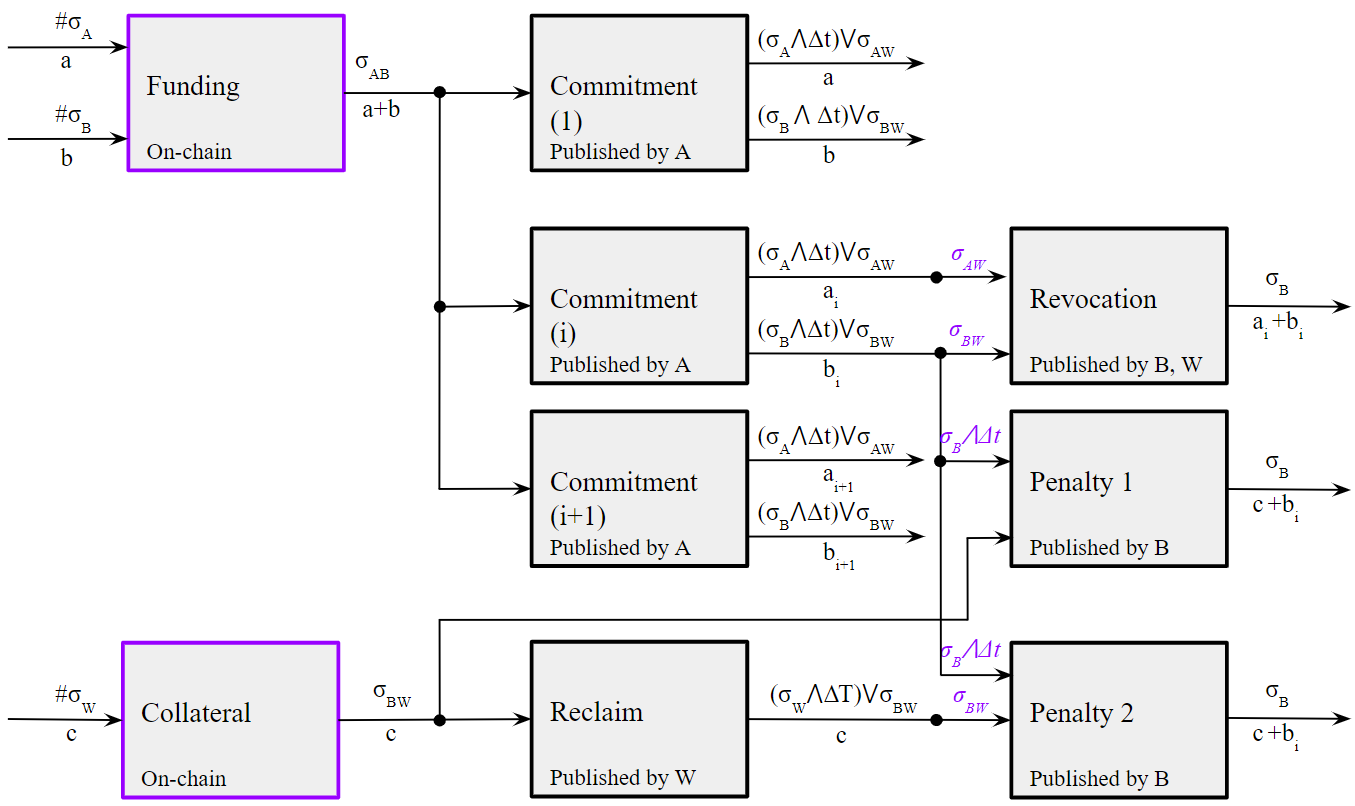
\includegraphics[width=\textwidth]{cerberous_it.PNG}
    % \includegraphics[scale=0.65]{test.PNG}
    % \caption{The transactions of a \sys channel and their dependencies. When many spending conditions are available in the output, the one used is explicitly shown emphasized in the input.}
    \caption{\sys channel transactions. When many spending conditions are available in the output, the one used is explicitly shown emphasized in the input.}
    \label{fig:txs}
\end{figure*}



% \begin{figure*}[ht!]
% 	\fbox{
% 	\begin{minipage}{0.97\textwidth}
% 	\begin{flushleft}
% 	\noindent\textbf{Protocol: \textsc{Abort}}\\
% 	\noindent\emph{Preconditions:} $W$ has $c$ coins locked as collateral for party $B$.
% 	\begin{enumerate}
% 	    \item $W$ spends on-chain the output of the collateral transaction $o_{Coll}$.
%         \end{enumerate}
%     \noindent\emph{Postconditions:} $W$ reclaims the collateral of $c$ coins (after time $T$ has elapsed since $W$ spent $o_{Coll}$ on-chain).
%         \end{flushleft}
% 	\end{minipage}
% 	}
% \caption{Watchtower terminates its employment by the channel party.}
% \label{prot:abort}
% \end{figure*}



%-------------------------------------------------
%---------------SECURITY ANALYSIS------------------------
%-------------------------------------------------
\section{Security Analysis}
% In this section, we show \sys channels achieve the protocol goals, \textit{Security} and \textit{Scale-out}.
% Further, we discuss \textit{Privacy}.

\subsection{Security}
We show that \sys channels are secure within our system model under any collusion/bribing scheme involving the channel parties and the watchtower.
%Omitted proofs can be found in Appendix \ref{sec:proofs}.


\begin{lemma}[Abort]\label{lem:abort}
Phase \textit{Abort} does not affect the security of a \sys channel, \ie, no honest party or watchtower can be cheated out of its funds.
% During phase \textit{Abort}, no honest party or watchtower can be cheated out of its funds.
\end{lemma}
\begin{proof}
To prove the lemma, we distinguish three cases:
\begin{enumerate}[label=(\alph*)]
    \item \textit{Abort} terminates before \textit{Close} initiates.
    \item \textit{Abort} terminates during \textit{Close}.
    \item \textit{Abort} includes \textit{Close} entirely, \ie, \textit{Close} initiates at most $T-t$ after the reclaim transaction is put on-chain.
\end{enumerate}

In the first case, the watchtower withdraws the collateral, and is not liable anymore for the channel operation.
Specifically, $W$ publishes on-chain the reclaim transaction. Since no commitment transaction is published on-chain, all penalty transactions that can interfere with the ownership of the collateral are invalid. Hence, the watchtower claims the collateral after time $T$ elapses -- before  \textit{Close} initiates.
From that point on, the security of the channel -- the funds of the hiring party -- is the same as in a Lightning channel, unless the channel is updated with a new watchtower service.

For the second case, suppose \textit{Abort} initiates at time $t=0$, and there is a time $t'$, such that $T-t < t'< T$, in which \textit{Close} initiates.
If the closing of the channel is collaborative between the parties or the last commitment transaction was published by one of the parties, there are no valid penalty transactions that can interfere with the ownership of the collateral. Hence, the collateral will be owned by the watchtower at time $T$.
Further, the funds of the channel parties will be distributed as last agreed.
However, the channel can close with one of the parties publishing an old commitment transaction.
In this case, both penalty transactions become valid at time $t'+t>T$. But the watchtower can spend the collateral at time $T$, before any penalty transaction becomes valid.
Therefore, when {Abort} terminates during \textit{Close}, the watchtower can safely reclaim the collateral, no matter how a \sys channel closes.
Note, however, that the watchtower is not liable for the channel's correct operation when {Abort} terminates during \textit{Close}.
Thus, the watchtower is not obligated to publish the revocation transaction in time.
% Nevertheless, the hiring party is online at least once every $T$ time.
% To be specific, the hiring party is either already aware of the published reclaim transaction, and thus will come online at least once very $t$ time, or will come online once until time $T$.
% Since $t'+t>T$, the hiring party will have the time to publish the revocation transaction.
Nevertheless, the hiring party comes online once during the \textit{Abort} phase. From then on, it comes online every $t$ time, since it realizes that the watchtower stops offering its service. Furthermore, it holds $t'+t>T$.
Therefore, the hiring party will notice the fraud in time and will publish the revocation transaction.
Hence, no honest hiring party or watchtower can be cheated out of its funds when {Abort} terminates during \textit{Close}.


In contrast to the first two cases, when \textit{Abort} includes \textit{Close} entirely, the watchtower is still responsible for the correct operation of the channel.
In such a case, the security of a \sys channel is the same with or without phase \textit{Abort}.
Thus, \textit{Abort} does not affect the security of a \sys channel.
\end{proof}


%Next, we show that any honest party will maintain at least its funds in a \sys channel, even against malicious parties.
\begin{lemma}[Collusion]\label{lem:collusion}
An honest \emph{\sys} member cannot be cheated out of its funds.
%Honest \emph{\sys} channel members cannot involuntarily lose funds.
\end{lemma}
\begin{proof}
Watchtowers are incentivized to participate in \sys channels due to the occasional rewards on every update.
Thus, we need only show that under any collusion scheme \sys channels remain secure with respect to the system model of Section~\ref{subsec:model}. This implies the scheme is also secure if no collusion occurs, \eg, normal channel operation or the watchtower is offline. Note that whenever we assume collusion, it can also be the case that the same person handles both colluding identities.
There can be the following collusion schemes:
\begin{enumerate}[label=(\roman*)]
    \item Both parties of the channel $A$ and $B$ collude.
    % This is equivalent to a single party creating a fake channel to defraud the watchtower.
    According to the cryptographic assumptions, the signature of the watchtower cannot be forged, hence the parties cannot create a penalty transaction without the collaboration of the watchtower.
    Moreover, the channel parties only hold the watchtower's signature for revocation and penalty transactions of previous commitment transactions. The reclaim transaction is only held by $W$ and phase \textit{Abort} does not affect the security of the protocol (Lemma \ref{lem:abort}). Therefore, the only available action for the colluding parties is to publish a previous commitment transaction on purpose. In such a case, an honest hence online watchtower publishes the corresponding revocation transaction. As soon as the revocation transaction is on-chain, one of the inputs of both penalty transactions -- which is the same as the one in the revocation transaction -- become invalid thus both penalty transaction become invalid. Therefore, the malicious parties cannot claim an honest watchtower's collateral.

    \item Watchtower $W$ colludes with party $A$.
    In this case, the malicious parties try to cheat $B$'s balance out of the channel (equivalent to at most $a+b$ coins), while $B$ is offline.
    We assume \textit{Abort} has not initiated, since it does not affect the security of the channel\footnote{To be precise, \textit{Abort} could have initiated but less than $T-t$ time has elapsed between the reclaim transaction was published on-chain and the time \textit{Close} initiated.} (Lemma \ref{lem:abort}).
    The colluding parties cannot forge $B$'s signature to close the channel in a new state. Thus, the only available action is to publish a previous and more favorable to $A$ commitment transaction.
    However, for each previous commitment transaction, party $B$ holds two corresponding penalty transactions that award the collateral of the watchtower to $B$. Therefore, as soon as $B$ goes online (within the time window $T$), $B$ will publish the suitable penalty transaction on-chain (type 2 if the reclaim transaction is on-chain, type 1 otherwise) and claim the watchtower's collateral, $c>a+b$ coins.
    Note that this argument holds because the watchtower's collateral is locked on-chain involving the hiring party and thus cannot be used in parallel for other channels/parties.

    \item In the last case, $B$ colludes with watchtower $W$.
    This is the simplest case, since $A$ is either online or employs its own watchtower. If $A$ is online the security holds similarly to the Lightning protocol, \ie, $A$ publishes the revocation transaction on-chain and receives all the funds of the channel. If $A$ employs a watchtower, then the previous analysis holds.
 \end{enumerate}
\end{proof}

\begin{lemma}[Correctness]\label{lem:correctness}
A \sys channel will not close in a state that is not the last state agreed by all the participants of the channel.
\end{lemma}
\begin{proof}
Any party of a \sys channel cannot gain more profit by deviating from the honest protocol execution, because all parties involved in a \sys channel always maintain (at least) their funds as shown in Lemma \ref{lem:collusion}. Hence, a rational party that aims to maximize its profit will honestly follow the \sys protocol in every phase, and ultimately close the \sys channel in a non-cheating state, as described in Section~\ref{sec:design}.
\end{proof}

\begin{lemma}[Time]\label{lem:time}
Any party of a \sys channel can close it at any time.
\end{lemma}
\begin{proof}
Both parties of the \sys channel hold at least one valid commitment transaction (the one created at the last execution of the Update protocol, or if no update has taken place, the unique commitment transaction created during the Open protocol) which allows them to initiate phase \textit{Close}, unilaterally, as described in Section~\ref{subsec:close}.
Hence, a \sys channel will be closed at the latest within time $t$ from publishing a commitment transaction on-chain (given a perfect underlying blockchain protocol and network synchrony).
\end{proof}


\begin{theorem}[Goals]
\sys channels achieve Security (as defined in Section~\ref{subsec:goals}).
\end{theorem}
\begin{proof}
Lemma~\ref{lem:time} states that any party can close a \sys channel at any time. From Lemma~\ref{lem:correctness}, it holds that a \sys channel can only close on the last agreed by all parties state. Hence, any party of a \sys channel can enforce the last agreed state on-chain at any time.
%From Lemma \ref{lem:time}, it holds that any party can close a \sys channel at any time. Thus, to prove %security it is enough to show that a \sys channel can only close on the last agreed by all parties state, %which is shown in Lemma \ref{lem:correctness}. Hence, any party of a \sys channel can enforce the last %agreed state on-chain at any time.
\end{proof}

\subsection{Performance}

Next, we show that \sys channels scale well, meaning that the number of on-chain transactions is constant and independent of the number of transactions executed in a channel, similarly to the Lightning protocol. The analysis below considers a single watchtower for each party of the channel. We discuss the scalability of the protocol if we enable multiple watchtowers in Section~\ref{sec:limit}.

\begin{theorem}[Scale]
\sys channels achieve Scale-out.
\end{theorem}
\begin{proof}
In phase \textit{Open}, a \sys channel requires $3$ transactions, one funding transaction to open the channel and two collateral transactions for each watchtower to lock the collateral to the corresponding party of the channel.
Phase \textit{Update} is executed off-chain, hence no transactions are published on-chain.

During phase \textit{Close}, the number of on-chain transactions can vary, however in the worst case $4$ transactions are published.
Specifically, in case of a non-cheating closure $3$ transactions are published: (i) either a commitment transaction published unilaterally by a party of the channel, or a collaborative closing transaction published by both parties, (ii)-(iii) one reclaim transaction for each of the parties' watchtowers, published by the corresponding watchtowers respectively.

On the contrary, in case of fraud and a responsive watchtower, the following $4$ transactions are necessary: (i) an old commitment transaction published by the cheating party (step 1, protocol \textsc{Close (B)}), (ii) the reclaim transaction of the cheating party's watchtower, published by the watchtower, (iii) the revocation transaction from the cheated party's watchtower, published by the watchtower (step 2, protocol \textsc{Close (B)}), and (iv) the reclaim transaction of the cheated party's watchtower, published by the watchtower (step 3, protocol \textsc{Close (B)}).

In case of fraud and an unresponsive watchtower, up to $4$ transactions are published on-chain, as illustrated in Protocol \textsc{Close (C)}: (i) an old commitment transaction published by the cheating party, (ii) the reclaim transaction of the cheating party's watchtower (published by the watchtower), (iii) the reclaim transaction of the cheated party's watchtower (published by the watchtower), and (iv) the corresponding penalty transaction published by the cheated party.

Phase \textit{Abort} is an optional intermediate phase that allows the watchtower to withdraw its service to the channel party. This phase includes one on-chain transaction -- the reclaim transaction -- but not additively to phase \textit{Close}. After phase \textit{Abort} the protocol for the party is similar to the Bitcoin Lightning protocol, which  requires at most $3$ on-chain transactions in total per channel. Thus, the worst case performance analysis does not include phase \textit{Abort}.

Overall, a \sys channel requires at most $7$ on-chain transactions.
\end{proof}


%-------------------------------------------------
%-------------------SCRIPT------------------------
%-------------------------------------------------
\section{Cerberus Transactions Script}
\label{sec:script}

Consider a channel between Alice and Bob, where only Bob is using a watchtower.
The funding and the collateral transactions both have a 2-of-2 multisig output. Their script is
\texttt{2 <pubkey1> <pubkey2> 2 OP\_CHECKMULTISIG},
where \texttt{pubkey1}, \texttt{pubkey2} are the funding keys of Alice and Bob for the funding transaction and the collateral keys of Bob and the watchtower for the collateral, sorted by ascending order of their DER-encodings\footnote{\url{https://github.com/bitcoin/bips/blob/master/bip-0066.mediawiki}}.

The reclaim transaction has one input that spends the collateral output with script
\texttt{0 <collateral\_pubkey1\_sig> <collateral\_pubkey2\_sig>}.
It has one output, with the script of Fig.~\ref{script:claim}. The public keys belong to Bob and the watchtower and are sorted by their DER-encodings.

% \begin{figure*}[ht!]
%     \begin{verbatim}
% OP_IF
%     # Penalty
%     2
%     <penalty_pubkey1>
%     <penalty_pubkey2>
%     2
%     OP_CHECKMULTISIG
% OP_ELSE
%     # Normal
%     <long_delay>
%     OP_CHECKSEQUENCEVERIFY
%     OP_DROP
%     <watchtower_penalty_pubkey>
%     OP_CHECKSIG
% OP_ENDIF
%     \end{verbatim}
% \caption{Reclaim transaction output script.}
% \label{script:claim}
% \end{figure*}

The commitment transaction has a unique input that spends the funding output with witness script \texttt{0 <pubkey1\_sig> <pubkey2\_sig>}. It also has two outputs, the scripts of which are slight variations of each other (replace Alice with Bob and vice-versa). Figure~\ref{script:commitment:first} depicts the first output, while
% The exact scripts can be found in Fig.~\ref{script:commitment:first} and~\ref{script:commitment:second}.
the exact scripts of both outputs can be found in the proof-of-concept implementation~\url{https://github.com/fc-submission-132/cerberus-script}.
For the first output, the two revocation public keys are those of Alice and the watchtower, sorted by ascending order of their DER-encodings. Similarly sorted are the revocation public keys of Bob and the watchtower in the second output.


\begin{figure}
\footnotesize
\begin{minipage}[ht]{0.45\textwidth}
 \begin{verbatim}OP_IF # Penalty
  2 <penalty_pubkey1>
  <penalty_pubkey2> 2
  OP_CHECKMULTISIG
OP_ELSE # Normal
  <long_delay>
  OP_CHECKSEQUENCEVERIFY
  OP_DROP
  <watchtower_penalty_pubkey>
  OP_CHECKSIG
OP_ENDIF\end{verbatim}
\caption{\footnotesize Reclaim transaction output script.}
\label{script:claim}
\end{minipage}
\hfill
\begin{minipage}[ht]{0.45\textwidth}
	\begin{verbatim}OP_IF # Revocation
  2 <revocation_pubkey1>
  <revocation_pubkey2> 2
  OP_CHECKMULTISIG
OP_ELSE # Normal
  <bob_delay>
  OP_CHECKSEQUENCEVERIFY
  OP_DROP
  <alice_delayed_pubkey>
  OP_CHECKSIG
OP_ENDIF\end{verbatim}
\caption{\footnotesize Commitment transaction 1st output script.}
\label{script:commitment:first}
\end{minipage}
% \hfill
% \begin{minipage}[ht]{0.45\textwidth}
% 	\begin{verbatim}
% OP_IF
%   # Revocation
%   2
%   <revocation_pubkey1>
%   <revocation_pubkey2>
%   2
%   OP_CHECKMULTISIG
% OP_ELSE
%   # Normal
%   <alice_delay>
%   OP_CHECKSEQUENCEVERIFY
%   OP_DROP
%   <bob_delayed_pubkey>
%   OP_CHECKSIG
% OP_ENDIF
%     \end{verbatim}
% \caption{\footnotesize Commitment transaction 2nd output script.}
% \label{script:commitment:second}
% \end{minipage}
\end{figure}

The revocation transaction spends the outputs of the commitment transaction following the revocation path. The witness script of both inputs is \texttt{0 <revocation\_pubkey1\_sig> <revocation\_pubkey2\_sig> 1} with the appropriate signatures for each output. It has a P2WPKH\footnote{\url{https://wiki.trezor.io/P2WPKH}} output to Bob's public key.

The penalty transaction 1 spends the second output of the commitment transaction and the output of the collateral transaction. It also has a single plain P2WPKH output to Bob's public key. The first input follows the normal path and has a witness script \texttt{<bob\_delayed\_pubkey\_sig> 0}, whereas the second input has a witness script \texttt{0 <collateral\_pubkey1\_sig> <collateral\_pubkey2\_sig>}.

Lastly, the penalty transaction 2 is similar to penalty transaction 1, but it spends the collateral instead of the reclaim transaction. Explicitly, penalty transaction 2 spends the 2nd output of the commitment and the output of the reclaim transaction following the penalty path. It has a single plain P2WPKH output to Bob's public key. The first input follows the normal path and has a witness script \texttt{<bob\_delayed\_pubkey\_sig> 0}, whereas the second input has a witness script \texttt{0 <penalty\_pubkey1\_sig> <penalty\_pubkey2\_sig> 1}.

% A proof-of-concept implementation of the necessary transactions can be found in
% \url{https://github.com/OrfeasLitos/cerberus-script}.

%-------------------------------------------------
%---------------FUTURE WORK AND LIMITATIONS-------------------
%-------------------------------------------------
\section{Limitations and future work}\label{sec:limit}
%  In this section, we discuss possible future work, extensions, and limitations of \sys channels.

% \paragraph{Privacy.}
\subsubsection*{Privacy.}
\sys channels maintain the privacy property, as defined in Section~\ref{subsec:goals}, assuming that the watchtowers are considered internal to the channel parties. This means that the transactions executed off-chain during the phase \textit{Update} are known only to the parties of the channel and the hired watchtowers. Any other third-party, external to the channel, does not have any knowledge on the state of the channel.
Nevertheless, \sys channels do not guarantee privacy from the watchtowers.
% Payment channels in Bitcoin offer by construction privacy of transactions on the channel, since all intermediate transactions are executed off-chain.
Although Lightning watchtowers preserve the privacy of transactions from watchtowers, they also suffer from inadequate incentives for participation in the system. On the other hand, \sys channels provide the necessary incentive mechanisms to guarantee security, but watchtowers are aware of all transactions executed in the channel.
Introducing stronger privacy mechanisms while maintaining the appropriate incentives is left for future work.

% \paragraph{Extension to multiple watchtowers.}
\subsubsection*{Extension to multiple watchtowers.}
To enhance security against possible crash failures or withdrawal of watchtower service, parties can employ many watchtowers. In such a case, every watchtower needs to lock its collateral on-chain, thus the number of on-chain transactions grows linearly with the number of watchtowers. However, to guarantee security, the sum of all watchtowers' collateral can remain the same, \ie, at least greater than the total funds locked in the channel by both parties. This way the counterparty of the channel cannot bribe all watchtowers since the sum of the required bribes will exceed the party's potential gain. Therefore, there will be at least one watchtower that will publish the revocation transaction in case of fraud.

% \paragraph{Rewards and Collateral.}
\subsubsection*{Rewards and Collateral.}
In the current system, rewards are awarded to the watchtowers on every update of the channel by the hired party via a one-way channel. Ideally, these rewards should be returned to the hired party if the watchtower misbehaves. To this end, we can modify the collateral transaction to build a bidirectional payment channel in which the watchtower locks collateral and the hirer locks future rewards. Then, during an update of the \sys channel and upon receiving the signed penalty transaction, the hirer sends some funds in this channel, paying the watchtower for its service. Note that this process does not require a fair exchange protocol since the watchtower can simply withdraw its service in case the hiring party does not pay the reward, similarly to the current protocol. However, this modification implies that the watchtowers' rewards will be locked during the lifetime of the channel.

% \paragraph{Assumptions.}
\subsubsection*{Assumptions.}
%  The security of \sys channels depends on synchrony assumptions
% and a perfect blockchain that cannot be censored. This is required due to timelocks. Although we enable shorter revocation periods and parties can go offline for an extended period of time, we cannot decouple the dependency of the security of payment channels on Bitcoin from the liveness and synchrony of the underlying blockchain.
% We believe that this is an inherent problem and limitation of the scripting language, since timelocks seem to be unavoidable.
In every channel construction that the counterparty is allowed to publish on-chain a valid outdated state, timelocks are necessary to secure the construction. Assuming distrusting parties (including the watchtower), this implies that every party must be online once in a while to verify the correct operation of the construction. Hence, at best we can alleviate the availability assumption, but not abolish it completely.
In turn, due to timelocks, the security of \sys channels depends on synchrony assumptions and a perfect blockchain that cannot be censored. Although we enable shorter revocation periods and parties can go offline for an extended period of time, we cannot decouple the dependency of the security of payment channels on Bitcoin from the liveness and synchrony of the underlying blockchain.



%-------------------------------------------------
%--------------BITCOIN IMPLEMENTATION------------------------
%-------------------------------------------------
% \section{Bitcoin Implementation}\label{sec:bitcoin}

% see appendixor github

% \url{https://github.com/OrfeasLitos/cerberus-script}


%-------------------------------------------------
%---------------RELATED WORK------------------------
%-------------------------------------------------
% \section{Related Work}
% \label{sec:related}

% Payment channels are the most prominent solution to the scalability problem of current blockchain systems. Payment channels were originally introduced by Spilman \cite{spilman2013channels} as unidirectional channels and were later established as bidirectional channels \cite{poon2015lightning,decker15fast}. Currently, there exist many different constructions of bidirectional payment channels, some applicable only on platforms that allow for arbitrary smart contracts such as Ethereum \cite{dziembowski2017perun,Miller2017sprites,green2017bolt,avarikioti2019brick}, and some applicable also on blockchain systems with limited scripting languages like Bitcoin \cite{poon2015lightning,deckereltoo,decker15fast,avarikioti2018watchtowers}. This work falls in the second category; we introduce \sys, a new payment channel construction, and provide a proof-of-concept implementation on Bitcoin.

% The most famous and active payment network is the Bitcoin Lightning network \cite{poon2015lightning} currently operating more than .... channels by over .... Bitcoin nodes \cite{}. However, Lighting as well as most of the other payment networks require channel parties that are constantly online, watching the blockchain. To address this issue, Dryja introduced Moritors \cite{dryja2016monitors}, also known as Watchtowers \cite{watchtowers}, a third party solution that acts as a proxy for a channel's party effectively allowing the party to go offline for a long period of time while maintaining the security of the channel operation (the other party cannot cheat). Watchtowers mainly focused on privacy preserving techniques to ensure the hired third-party does not learn any information about the off-chain transactions.
% Thereafter, Avarikioti et al.\ proposed DCWC \cite{avarikioti2018watchtowers}, a distributed protocol for watchtower services, in an attempt to involve all full nodes to participate in the system and consequently enhance security.
% However, both these works, Watchtowers and DCWC, fail to provide the necessary incentives for participation in the system. In particular, if a party hires a Watchtower and pays him regularly, the Watchtower has no incentive to do its job (since he is being paid regardless). On the other hand, if the Watchtower is being paid when fraud occurs, he will not participate in this system because no rational party will commit fraud hence he will never be paid. On the contrary, \sys channels provide the necessary incentives mechanisms, \ie, penalization of the watchtower's collateral in addition to the occasional rewards.

% Towards the same direction, McCorry et al.\ presented Pisa \cite{mccorry2018pisa}, a protocol that outsources the dispute handling of (state\footnote{State channels are a generalization of payment channels that support smart contracts \cite{Miller2017sprites}.}) channels to hired third-parties. However, Pisa has two shortcomings: First, the main protocol implementation is not secure against bribing since the watchtower's collateral is not linked to the party or the channel on-chain, hence the watchtower can double-spend it. Second, Pisa is not compatible with Bitcoin, because it requires a smart contract beyond the limitations of script. On the contrary, \sys channels are applicable on Bitcoin and furthermore they do not suffer from the security problems of Pisa since the watchtower locks the collateral linked to the hiring party on-chain.

% More recently, Avarikioti et al.\ introduced Brick~\cite{avarikioti2019brick}, an asynchronous off-chain construction that utilizes a committee of watchtowers. Although Brick manages to remove the synchrony requirements on the network layer and the perfect blockchain assumption while maintaining the security of payment channels, it is not compatible with Bitcoin-like platforms. In this work we provide a proof-of concept implementation on Bitcoin, which can be found in appendix  \ref{sec:script}.

% In a different line of work, Khabbazian  et al.~\cite{khabbazian2019outpost} proposed a lightweight watchtower design in which watchtowers do not need to store the signed justice (revocation) transactions, but instead can extract them  directly from the commitment transactions that appear on the blockchain.
% This work is independent and complementary to ours, and can be applied also to \sys channels to improve the storage requirements for the watchtower service.
% % This work is independent to ours, since it considers the original watchtower proposal \cite{dryja2016monitors} that due to privacy reasons
% % requires large storage and lookup time for the watchtower.
% % In contrast, off-chain transactions in \sys are not hidden from then watchtowers.

%-------------------------------------------------
%---------------CONCLUSION------------------------
%-------------------------------------------------
% \section{Conclusion}
% \label{sec:conclusion}

\bibliographystyle{abbrv}
\bibliography{net,sec,os,ref}

% \iffalse
\newpage

\appendix

\iffalse
\section{Omitted proofs}\label{sec:proofs}

\abort*
\begin{proof}
To prove the lemma, we distinguish three cases:
\begin{enumerate}[label=(\alph*)]
    \item \textit{Abort} terminates before \textit{Close} initiates.
    \item \textit{Abort} terminates during \textit{Close}.
    \item \textit{Abort} includes \textit{Close} entirely, \ie, \textit{Close} initiates at most $T-t$ after the reclaim transaction is put on-chain.
\end{enumerate}

In the first case, the watchtower withdraws the collateral, and is not liable anymore for the channel operation.
Specifically, $W$ publishes on-chain the reclaim transaction. Since no commitment transaction is published on-chain, all penalty transactions that can interfere with the ownership of the collateral are invalid. Hence, the watchtower claims the collateral after time $T$ elapses -- before  \textit{Close} initiates.
From that point on, the security of the channel -- the funds of the hiring party -- is the same as in a Lightning channel, unless the channel is updated with a new watchtower service.

For the second case, suppose \textit{Abort} initiates at time $t=0$, and there is a time $t'$, such that $T-t < t'< T$, in which \textit{Close} initiates.
If the closing of the channel is collaborative between the parties or the last commitment transaction was published by one of the parties, there are no valid penalty transactions that can interfere with the ownership of the collateral. Hence, the collateral will be owned by the watchtower at time $T$.
Further, the funds of the channel parties will be distributed as last agreed.
However, the channel can close with one of the parties publishing an old commitment transaction.
In this case, both penalty transactions become valid at time $t'+t>T$. But the watchtower can spend the collateral at time $T$, before any penalty transaction becomes valid.
Therefore, when {Abort} terminates during \textit{Close}, the watchtower can safely reclaim the collateral, no matter how a \sys channel closes.
Note, however, that the watchtower is not liable for the channel's correct operation when {Abort} terminates during \textit{Close}.
Thus, the watchtower is not obligated to publish the revocation transaction in time.
% Nevertheless, the hiring party is online at least once every $T$ time.
% To be specific, the hiring party is either already aware of the published reclaim transaction, and thus will come online at least once very $t$ time, or will come online once until time $T$.
% Since $t'+t>T$, the hiring party will have the time to publish the revocation transaction.
Nevertheless, the hiring party comes online once during the \textit{Abort} phase. From then on, it comes online every $t$ time, since it realizes that the watchtower stops offering its service. Furthermore, it holds $t'+t>T$.
Therefore, the hiring party will notice the fraud in time and will publish the revocation transaction.
Hence, no honest hiring party or watchtower can be cheated out of its funds when {Abort} terminates during \textit{Close}.


In contrast to the first two cases, when \textit{Abort} includes \textit{Close} entirely, the watchtower is still responsible for the correct operation of the channel.
In such a case, the security of a \sys channel is the same with or without phase \textit{Abort}.
Thus, overall, \textit{Abort} does not affect the security of a \sys channel.
\end{proof}

 Next, we show that any honest party will maintain at least its funds in a \sys channel, even against malicious parties.
\collusion*
\begin{proof}
Watchtowers are incentivized to participate in \sys channels due to the occasional rewards on every update.
Thus, we need only show that under any collusion scheme \sys channels remain secure with respect to the system model of Section~\ref{subsec:model}. This implies the scheme is also secure if no collusion occurs, \eg, normal channel operation or the watchtower is offline. Note that whenever we assume collusion, it can also be the case that the same person handles both colluding identities.
There can be the following collusion schemes:
\begin{enumerate}[label=(\roman*)]
    \item Both parties of the channel $A$ and $B$ collude.
    % This is equivalent to a single party creating a fake channel to defraud the watchtower.
    According to the cryptographic assumptions, the signature of the watchtower cannot be forged, hence the parties cannot create a penalty transaction without the collaboration of the watchtower.
    Moreover, the channel parties only hold the watchtower's signature for revocation and penalty transactions of previous commitment transactions. The reclaim transaction is only held by $W$ and phase \textit{Abort} does not affect the security of the protocol (Lemma \ref{lem:abort}). Therefore, the only available action for the colluding parties is to publish a previous commitment transaction on purpose. In such a case, an honest hence online watchtower publishes the corresponding revocation transaction. As soon as the revocation transaction is on-chain, one of the inputs of both penalty transactions -- which is the same as the one in the revocation transaction -- become invalid thus both penalty transaction become invalid. Therefore, the malicious parties cannot claim an honest watchtower's collateral.

    \item Watchtower $W$ colludes with party $A$.
    In this case, the malicious parties try to cheat $B$'s balance out of the channel (equivalent to at most $a+b$ coins), while $B$ is offline.
    We assume \textit{Abort} has not initiated, since it does not affect the security of the channel\footnote{To be precise, \textit{Abort} could have initiated but less than $T-t$ time has elapsed between the reclaim transaction was published on-chain and the time \textit{Close} initiated.} (Lemma \ref{lem:abort}).
    The colluding parties cannot forge $B$'s signature to close the channel in a new state. Thus, the only available action is to publish a previous and more favorable to $A$ commitment transaction.
    However, for each previous commitment transaction, party $B$ holds two corresponding penalty transactions that award the collateral of the watchtower to $B$. Therefore, as soon as $B$ goes online (within the time window $T$), $B$ will publish the suitable penalty transaction on-chain (type 2 if the reclaim transaction is on-chain, type 1 otherwise) and claim the watchtower's collateral, $c>a+b$ coins.
    Note that this argument holds because the watchtower's collateral is locked on-chain involving the hiring party and thus cannot be used in parallel for other channels/parties.

    \item In the last case, $B$ colludes with watchtower $W$.
    This is the simplest case, since $A$ is either online or employs its own watchtower. If $A$ is online the security holds similarly to the Lightning protocol, \ie, $A$ publishes the revocation transaction on-chain and receives all the funds of the channel. If $A$ employs a watchtower, then the previous analysis holds.
 \end{enumerate}
\end{proof}


\correctness*
\begin{proof}
Any party of a \sys channel cannot gain more profit by deviating from the honest protocol execution, because all parties involved in a \sys channel always maintain (at least) their funds as shown in Lemma \ref{lem:collusion}. Hence, a rational party that aims to maximize its profit will honestly follow the \sys protocol in every phase, and ultimately close the \sys channel in a non-cheating state, as described in Section~\ref{sec:design}.
\end{proof}

\time*
\begin{proof}
Both parties of the \sys channel hold at least one valid commitment transaction (the one created at the last execution of the Update protocol, or if no update has taken place, the unique commitment transaction created during the Open protocol) which allows them to initiate phase \textit{Close}, unilaterally, as described in Section~\ref{subsec:close}.
Hence, a \sys channel will be closed at the latest within time $t$ from publishing a commitment transaction on-chain (given a perfect underlying blockchain protocol and network synchrony).
\end{proof}

% \goals*
% \begin{proof}
% From Lemma \ref{lem:time}, it holds that any party can close a \sys channel at any time. Thus, to prove security it is enough to show that a \sys channel can only close on the last agreed by all parties state, which is shown in Lemma \ref{lem:correctness}. Hence, any party of a \sys channel can enforce the last agreed state on-chain at any time.
% \end{proof}

The analysis below considers a single watchtower for each channel party.

\scale*
\begin{proof}
In phase \textit{Open}, a \sys channel requires $3$ transactions, one funding transaction to open the channel and two collateral transactions for each watchtower to lock the collateral to the corresponding party of the channel.

Phase \textit{Update} is executed off-chain, hence no transactions are published on-chain.

During phase \textit{Close}, the number of on-chain transactions can vary, however in the worst case $4$ transactions are published.
Specifically, in case of a non-cheating closure $3$ transactions are published: (i) either a commitment transaction published unilaterally by a party of the channel, or a collaborative closing transaction published by both parties, (ii)-(iii) one reclaim transaction for each of the parties' watchtowers, published by the corresponding watchtowers respectively.

On the contrary, in case of fraud and a responsive watchtower, the following $4$ transactions are necessary: (i) an old commitment transaction published by the cheating party (step 1, protocol \textsc{Close (B)}), (ii) the reclaim transaction of the cheating party's watchtower, published by the watchtower, (iii) the revocation transaction from the cheated party's watchtower, published by the watchtower (step 2, protocol \textsc{Close (B)}), and (iv) the reclaim transaction of the cheated party's watchtower, published by the watchtower (step 3, protocol \textsc{Close (B)}).

Furthermore, in case of fraud and an unresponsive watchtower, up to $4$ transactions are published on-chain, as illustrated in Protocol \textsc{Close (C)}: (i) an old commitment transaction published by the cheating party, (ii) the reclaim transaction of the cheating party's watchtower (published by the watchtower), (iii) the reclaim transaction of the cheated party's watchtower (published by the watchtower), and (iv) the corresponding penalty transaction published by the cheated party.

Phase \textit{Abort} is an optional intermediate phase, that allows the watchtower to withdraw its service to the channel party. This phase includes one on-chain transaction -- the reclaim transaction -- but not additively to phase \textit{Close}. After phase \textit{Abort} the protocol for the party is similar to the Bitcoin Lightning protocol, which  requires at most $3$ on-chain transactions in total for a channel operation. Thus, the worst case performance analysis does not include phase \textit{Abort}.

Overall, a \sys channel requires at most $7$ on-chain transactions.
\end{proof}


%-------------------------------------------------
%-------------------SCRIPT------------------------
%-------------------------------------------------
\section{Cerberus transactions script}
\label{sec:script}

In the following specification we assume a channel between Alice and Bob, where only Bob is using a watchtower.
The funding and the collateral transactions both have a 2-of-2 multisig output. Its script is
\texttt{2 <pubkey1> <pubkey2> 2 OP\_CHECKMULTISIG},
where \texttt{pubkey1}, \texttt{pubkey2} are the funding public keys of Alice and Bob for the funding transaction and the collateral public keys of Bob and the watchtower, sorted by ascending order of their DER-encodings\footnote{\url{https://github.com/bitcoin/bips/blob/master/bip-0066.mediawiki}}.

The reclaim transaction has a unique input that spends the collateral transaction multisig output with a witness script
\texttt{0 <collateral\_pubkey1\_sig> <collateral\_pubkey2\_sig>}.
It also has a single output, with the script of Fig.~\ref{script:claim}. The two public keys belong to Bob and the watchtower and are sorted by their DER-encodings.

\begin{figure*}[ht!]
    \begin{verbatim}
OP_IF
    # Penalty
    2
    <penalty_pubkey1>
    <penalty_pubkey2>
    2
    OP_CHECKMULTISIG
OP_ELSE
    # Normal
    <long_delay>
    OP_CHECKSEQUENCEVERIFY
    OP_DROP
    <watchtower_penalty_pubkey>
    OP_CHECKSIG
OP_ENDIF
    \end{verbatim}
\caption{Reclaim transaction output script.}
\label{script:claim}
\end{figure*}

The commitment transaction has a unique input that spends the funding output with witness script \texttt{0 <pubkey1\_sig> <pubkey2\_sig>}. It also has two outputs, the scripts of which are slight variations of each other. The exact scripts can be found in Fig.~\ref{script:commitment:first} and~\ref{script:commitment:second}.

For the first output, the two revocation public keys are those of Alice and the watchtower, sorted by ascending order of their DER-encodings. Similarly sorted are the revocation public keys of Bob and the watchtower in the second output.

\begin{figure*}[ht!]
	\begin{verbatim}
OP_IF
    # Revocation
    2
    <revocation_pubkey1>
    <revocation_pubkey2>
    2
    OP_CHECKMULTISIG
OP_ELSE
    # Normal
    <bob_delay>
    OP_CHECKSEQUENCEVERIFY
    OP_DROP
    <alice_delayed_pubkey>
    OP_CHECKSIG
OP_ENDIF
    \end{verbatim}
\caption{Commitment transaction 1st output script.}
\label{script:commitment:first}
\end{figure*}

\begin{figure*}[ht!]
	\begin{verbatim}
OP_IF
    # Revocation
    2
    <revocation_pubkey1>
    <revocation_pubkey2>
    2
    OP_CHECKMULTISIG
OP_ELSE
    # Normal
    <alice_delay>
    OP_CHECKSEQUENCEVERIFY
    OP_DROP
    <bob_delayed_pubkey>
    OP_CHECKSIG
OP_ENDIF
    \end{verbatim}
\caption{Commitment transaction 2nd output script.}
\label{script:commitment:second}
\end{figure*}

The revocation transaction spends the two outputs of the commitment transaction following the revocation path. The witness script of both inputs is \texttt{0 <revocation\_pubkey1\_sig> <revocation\_pubkey2\_sig> 1} with the appropriate signatures for each output. It has a single P2WPKH\footnote{\url{https://wiki.trezor.io/P2WPKH}} output to Bob's public key.

The penalty transaction 1 spends the second output of the commitment transaction and the output of the collateral transaction. It also has a single plain P2WPKH output to Bob's public key. The first input follows the normal path and has a witness script \texttt{<bob\_delayed\_pubkey\_sig> 0}, whereas the second input has a witness script \texttt{0 <collateral\_pubkey1\_sig> <collateral\_pubkey2\_sig>}.

Lastly, the penalty transaction 2 is very similar with penalty transaction 1, except that does not spend the collateral, but the reclaim transaction. Explicitly, penalty transaction 2 spends the second output of the commitment transaction and the output of the reclaim transaction following the penalty path. It also has a single plain P2WPKH output to Bob's public key. The first input follows the normal path and has a witness script \texttt{<bob\_delayed\_pubkey\_sig> 0}, whereas the second input has a witness script \texttt{0 <penalty\_pubkey1\_sig> <penalty\_pubkey2\_sig> 1}.

A proof-of-concept implementation of the necessary transactions can be found in
\url{https://github.com/fc-submission-132/cerberus-script}.
% \url{https://github.com/fc-submission-132/cerberus-script}.
 \fi

\end{document}
